\documentclass[punct=kaiming,fontset=none]{ctexart}
\usepackage[a4paper,textwidth=462bp,vmargin=2cm]{geometry}
\usepackage{amsmath,amsthm,unicode-math}
\usepackage{siunitx}
\usepackage{xeCJKfntef}
\setmainfont{XITS}
\usepackage{sourcesanspro,sourcecodepro}
\setmathfont{XITS Math}
\setCJKmainfont{Source Han Serif CN}[
  UprightFont    = *-Regular,
  BoldFont       = *-Bold,
  ItalicFont     = 方正新楷体简体,
  BoldItalicFont = *-Bold,
  Mapping        = fullwidth-stop
]
\setCJKsansfont{Source Han Sans CN}
\setCJKmonofont{Source Han Sans CN}
\theoremstyle{definition}
\newtheorem{ti}{}[section]
\newtheorem*{solution}{解}
\renewcommand{\theti}{\arabic{ti}}
\RequirePackage{enumitem,calc}
\setlist[enumerate,1]{leftmargin=0pt,labelsep=0pt,itemindent=3\ccwd+0.05cm,parsep=0pt,itemsep=0pt,topsep=0pt,partopsep=0pt,listparindent=2\ccwd}
\def\labelenumi{(\theenumi)}
\usepackage{caption}
\usepackage{tikz}
\usetikzlibrary{decorations.markings}

\makeatletter
\newcommand{\fourch}[4]{%
  \noindent%
  \begin{tabular}{*{4}{@{}p{0.25\textwidth}@{}}}%
    \@hangfrom{\textsf A.}#1 & \@hangfrom{\textsf B.}#2 & \@hangfrom{\textsf C.}#3 & \@hangfrom{\textsf D.}#4
  \end{tabular}%
}
\newcommand{\twoch}[4]{%
  \noindent%
  \begin{tabular}{*{2}{@{}p{0.5\textwidth}@{}}}%
    \@hangfrom{\textsf A.}#1 & \@hangfrom{\textsf B.}#2 \\
    \@hangfrom{\textsf C.}#3 & \@hangfrom{\textsf D.}#4
  \end{tabular}%
}
\newcommand{\onech}[4]{%
  \noindent%
  \begin{tabular}{@{}p{\textwidth}@{}}%
    \@hangfrom{\textsf A.}#1 \\
    \@hangfrom{\textsf B.}#2 \\
    \@hangfrom{\textsf C.}#3 \\
    \@hangfrom{\textsf D.}#4
  \end{tabular}%
}
\makeatother
\usepackage[colorlinks=true,bookmarksopen=true,bookmarksnumbered=true]{hyperref}

\def\out{\mathrm{out}}
\def\REF{\mathrm{REF}}
\def\mm{\mathrm{m}}
\def\ee{\mathrm{e}}
\let\siold\si
\let\SIold\SI
\renewcommand{\si}[1]{\mbox{\siold{#1}}}
\renewcommand{\SI}[2]{\mbox{\SIold{#1}{#2}}}
\def\xiahua#1{\CJKunderline[hidden=false]{#1}}
\def\xiahuaa#1{\CJKunderline*[hidden=false]{#1}}
\def\kuohao#1{(\nobreak\textsf{#1}\nobreak)}
\title{《计算机控制技术》 2019--2020 考试卷\thanks{试卷编号:1920020605B}}
\author{\url{https://github.com/sikouhjw/jxust-Learning-database}}
\begin{document}
\maketitle
\section{填空题(每空2分,共20分)}
\begin{ti}
现有的两种硬件消抖电路是\xiahua{积分电路、R-S 触发器}。
\end{ti}
\begin{ti}
$V_{\out}$ 为 8 位 D/A 转换器的双极性输出端,若输入数字量 $\mathrm{D}=\SI{10100000}{B}$,基准参考电压 $V_{\REF} = \SI{5}{V}$,则 $V_{\out}$ 为\xiahua{ \SI{1.25}{V}}。
\end{ti}
\begin{ti}
第三象限逆圆弧插补,当偏差 $F_{\mm} < 0$ 时,下一步的进给方向为\xiahua{ $-y$}。
\end{ti}
\begin{ti}
将连续控制器 $D(s)$ 离散化为数字控制器 $D(z)$ 的方法有很多,其中用\xiahua{ $s = (z-1)/(Tz)$ }表示后向差分法由 $D(s)$ 求取 $D(z)$ 的计算公式。
\end{ti}
\begin{ti}
在 PID 控制系统中,P 的作用主要是\xiahuaa{迅速反应误差,从而减小误差}。
\end{ti}
\begin{ti}\label{ti:6}
如图~\ref{fig:6} 所示的数字 PID 控制器的改进为\xiahua{不完全微分}。
\begin{figure}[!htbp]
\centering
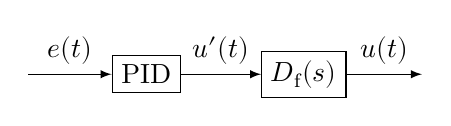
\begin{tikzpicture}
  \node[draw=black] (a) at (0,0) {PID};
  \node[draw=black] (b) at (2,0) {$D_{\mathrm{f}}(s)$};
  \draw[latex-] (a) -- node[above] {$e(t)$} ++ (-1.5,0);
  \draw[-latex] (a) -- node[above] {$u'(t)$} ++ (b);
  \draw[-latex] (b) -- node[above] {$u(t)$} ++ (1.5,0);
\end{tikzpicture}
\caption{填空题第~\ref{ti:6} 题的图}\label{fig:6}
\end{figure}
\end{ti}
\begin{ti}
消除振铃的方法是\xiahua{消除振铃因子法、参数选择法}。
\end{ti}
\begin{ti}
现已知某飞机飞行高度变化范围为 $0 \sim 15000$ 米,测试时,采用 12 位的 A/D 变换器,试问此时系统对高度变化的分辨率为\xiahua{ 3.66 }米。
\end{ti}
\section{选择题(每空2分,共20分)}
\begin{ti}
DCS 从下到上分为分散过程控制级、\kuohao{A}、综合信息管理级,形成分级分布式控制。

\fourch{集中操作监控级}{生产执行系统级}{自动处理操作级}{信息维护发送级}
\end{ti}
\begin{ti}
以下选项中不是共模干扰的抑制方式的是\kuohao{C}。

\fourch{光电隔离}{变压器隔离}{提高回路噪声比}{浮地屏蔽}
\end{ti}
\begin{ti}
当尖峰型串模干扰成为主要干扰源时,用\kuohao{C}可以削弱串模干扰的影响。

\fourch{低通滤波器}{高通滤波器}{双积分式 A/D 转换器}{变压器隔离}
\end{ti}
\begin{ti}
在步进电机控制模型中,不属于三相单三拍工作方式下的输出字表是\kuohao{D}。

\fourch{\SI{01}{H}}{\SI{02}{H}}{\SI{04}{H}}{\SI{06}{H}}
\end{ti}
\begin{ti}
下面不属于积分项的改进的是\kuohao{A}。

\fourch{分段积分}{抗积分饱和}{梯形积分}{消除积分不灵敏区}
\end{ti}
\begin{ti}
如果针对速度输入函数进行设计,为了跟踪输入,稳态过程中 $G_c(s)$ 的输出也必须是速度函数,为了产生这样的速度输出函数,$G_c(s)$ 中必须至少有\kuohao{A}个积分环节,使得控制信号 $u(k)$ 为常值(包括零)时,$G_c(s)$ 的稳态输出是所要求的速度函数。

\fourch{1}{2}{3}{4}
\end{ti}
\begin{ti}
某控制系统中,希望快速采样,保持器的保持电容 CH 应取值\kuohao{A}。

\fourch{比较小}{比较大}{取零值}{取负值}
\end{ti}
\begin{ti}
以下选项中不是整定PID参数的方法的是\kuohao{D}。

\fourch{扩充临界比例度法}{扩充响应曲线}{归一参数整定法}{经验法}
\end{ti}
\begin{ti}
下面关于标度变换的说法正确的是\kuohao{C}。

\onech{标度变换就是数字量变成工程量}{标度变换是把数字量变成工程量相关的模拟量}{标度变换就是把数字量转换成众所熟悉的十进制工程量}{以上说法都不对}
\end{ti}
\begin{ti}
能有效克服因偶然因素引起的波动干扰的滤波方法是\kuohao{C}。

\fourch{平均值滤波}{滑动平均滤波}{中位值滤波}{惯性滤波}
\end{ti}

\section{简答题(每小题5分,共10分)}
\begin{ti}
解释下面几个常用英文缩略语IPC,DDC,DCS,FCS,PCS的意思。
\begin{solution}
  IPC:工控机;
  DDC:直接数字控制系统;
  DCS:集散控制系统;
  FCS:现场总线控制系统;
  PCS:生产过程控制系统。
\end{solution}

\end{ti}
\begin{ti}
在工业控制系统中,常采用PID控制,试写出数字PID控制器的位置型控制算法和增量型控制算法的表达式。
\begin{solution}
  数字 PID 控制器的位置型控制算法:
  \[ u(k) = K_{\mathrm{P}} \left[ e(k) + \frac{T}{T_{\mathrm{I}}} \sum_{i=0}^k e(i) + T_{\mathrm{D}} \frac{e(k) - e(k-1)}{T} \right] \]
  数字 PID 控制器的增量型控制算法:
  \[ \Delta u(k) = K_{\mathrm{P}} [e(k) - e(k-1)] + K_{\mathrm{I}} e(k) + K_{\mathrm{D}} [e(k) - 2e(k-1) + e(k-2)] \]
  式中,$K_{\mathrm{P}}$ 为比例增益,$K_{\mathrm{P}} = 1/\sigma$;$K_{\mathrm{I}}$ 为积分系数,$K_{\mathrm{I}} = K_{\mathrm{P}} T/T_{\mathrm{I}}$;$K_{\mathrm{D}}$ 为微分系数,$K_{\mathrm{D}} = K_{\mathrm{P}} T_{\mathrm{D}}/T$。
\end{solution}
\end{ti}

\section{作图题(10分)}
\begin{ti}
设加工第二象限内一直线 $OA$,起点为 $O(0,0)$,终点为 $A(-5,3)$,试用逐点比较法进行插补计算,插补计算过程列表,并画出走步轨迹图并标明进给方向和步数。
\begin{solution}
坐标进给的总步数 $N_{xy} = |-5-0| + |3-0| = 8$,$x_{\ee} = 5$,$y_{\ee} = 3$,$F_0 = 0$,$xOy = 2$,插补计算过程见表~\ref{tab:1}。
\begin{table}[!htbp]
\centering
\caption{}\label{tab:1}
\begin{tabular}{c*{3}{|c}|c}
  \hline
  步数 & 偏差判别 & 坐标进给 & 偏差计算 & 终点判断 \\
  \hline
  起点 & & & $F_0=0$ & $N_{xy}=8$ \\
  \hline
  1 & $F_0=0$ & $-x$ & $F_1 = F_0 - y_\ee = -3$ & $N_{xy}=7$ \\
  \hline
  2 & $F_1<0$ & $+y$ & $F_2 = F_1 + x_\ee = 2$ & $N_{xy}=6$ \\
  \hline
  3 & $F_2>0$ & $-x$ & $F_3 = F_2 - y_\ee = -1$ & $N_{xy}=5$ \\
  \hline
  4 & $F_3<0$ & $+y$ & $F_4 = F_3 + x_\ee = 4$ & $N_{xy}=4$ \\
  \hline
  5 & $F_4>0$ & $-x$ & $F_5 = F_4 - y_\ee = 1$ & $N_{xy}=3$ \\
  \hline
  6 & $F_5>0$ & $-x$ & $F_6 = F_5 - y_\ee = -2$ & $N_{xy}=2$ \\
  \hline
  7 & $F_6<0$ & $+y$ & $F_7 = F_6 + x_\ee = 3$ & $N_{xy}=1$ \\
  \hline
  8 & $F_7>0$ & $-x$ & $F_8 = F_7 - y_\ee = 0$ & $N_{xy}=0$ \\
  \hline
\end{tabular}
\end{table}
\newcounter{jishu}
\setcounter{jishu}{1}
\def\xx{-- node[below] {\footnotesize\thejishu\stepcounter{jishu}} ++ (-1,0)}
\def\yy{-- node[right] {\footnotesize\thejishu\stepcounter{jishu}} ++ (0,1)}

直线插补的走步轨迹图如图~\ref{fig:4-1} 所示。
\begin{figure}[!htbp]
\centering
\begin{tikzpicture}[decoration={markings,mark=between positions 0 and 1 step 10mm with {\fill (0,0) circle (0.05);}}]
  \draw[-latex] (0,0) -- ++ (0,4) node[right] {$y$};
  \draw[-latex] (-6,0) -- ++ (7,0) node[above] {$x$};
  \draw (0,0) -- ++ (-5,3);
  \draw[-latex,postaction={decorate}] (0,0) \xx\yy\xx\yy\xx\xx\yy\xx;
  \foreach \x in {0,...,-5} {\draw (\x,0) -- ++ (0,0.2);\node[below] at (\x,0) {$\x$};}
  \foreach \y in {1,...,3} {\draw (0,\y) -- ++ (0.2,0);\node[left] at (0,\y) {$\y$};}
\end{tikzpicture}
\caption{}\label{fig:4-1}
\end{figure}
\end{solution}
\end{ti}

\section{设计题(15分)}
\begin{ti}
用8位A/D转换器ADC0809与PC/ISA总线工业控制机接口,实现8路模拟量采集。请画出接口原理图,并设计出8路模拟量的数据采集程序。
\begin{solution}
  略。
\end{solution}
\end{ti}

\section{计算题(25分)}
\begin{ti}
已知模拟调节器的传递函数为 $D(s) = \frac{1+0.2s}{1+0.09s}$,试写出相应数字控制器的位置型和增量型控制算式,设采样周期 $T = \SI{0.2}{s}$。(10分)
\begin{solution}
  由于 \[D(s) = \frac{U(s)}{E(s)} = \frac{1+0.2s}{1+0.09s},\]
  则 \[ u(k) + 0.09 \frac{u(k) - u(k-1)}{T} = e(k) + 0.2 \frac{e(k) - e(k-1)}{T}. \]
  把 $T = \SI{0.2}{s}$ 代入得位置型控制算法为 \[ u(k) = 0.31 u(k-1) + 1.38 e(k) - 0.69 e(k-1), \]
  则 \[ u(k-1) = 0.31 u(k-2) + 1.38 e(k-1) - 0.69 e(k-2). \]
  增量型控制算式为 \[ \Delta u(k) = u(k) - u(k-1) = 0.31 \Delta u(k-1) + 1.38 e(k) - 2.07 e(k-1) + 0.69 e(k-2). \]
\end{solution}
\end{ti}
\begin{ti}
己知广义对象的脉冲传递函数为:\[ G(z) = \frac{3.679z^{-1}(1+0.718z^{-1})}{(1-z^{-1})(1-0.3679z^{-1})} \]
\begin{enumerate}
  \item 用最小拍无纹波系统的设计方法,设计单位阶跃输入时闭环脉冲传递函数 $\varPhi(z)$ 和最少拍控制器 $D(z)$;
  \item 求出数字控制器输出序列 $u(k)$ 的递推形式;
  \item 画出采样瞬间数字控制器的输出和系统的输出曲线。(15分)
\end{enumerate}
\begin{solution}
  略。
\end{solution}
\end{ti}
\end{document}